\documentclass[11pt]{article}
\title{Meccano hexagons gallery}
\author{https://github.com/heptagons/meccano/hexa/gallery}
\date{2023/12/27}

\usepackage{../../meccano}
\usepackage{amssymb}
\usepackage{subcaption}


\begin{document}

\maketitle
\begin{abstract}
We build meccano\meccanoref rigid regular heptagons.
\end{abstract}

\section{Heptagon internals}

\begin{figure}[h]
\centering
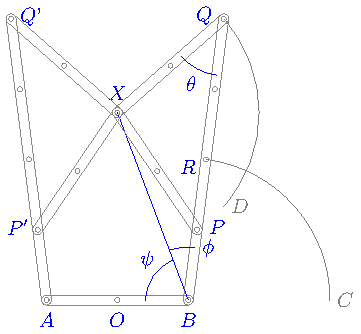
\includegraphics[scale=1.1]{builder/hepta-base}
\caption{Cluster of four strips with fixed vertices $A$ at $(-1,0)$, $B$ at $(+1,0)$ and $X$ at $(0,\sqrt7)$.}
\label{fig:build-base}
\end{figure}

Figure \ref{fig:build-base} show a cluster to make a triangle $\triangle{ABX}$ useful to make a regular heptagon. With the law of cosines we calculate first the angle $\theta \equiv \angle{PQX}$ and then the distance $\overline{BX}$:
\begin{align}
\cos\theta &= \frac{(\overline{PQ})^2 + (\overline{QX})^2 - (\overline{XP})^2}
 {2(\overline{PQ})(\overline{QX})} 
 = \frac{3^2 + 2^2 - 2^2}{2(3)(2)} = \frac{3}4 \label{eq:theta} \\
\overline{BX} &= \sqrt{(\overline{BQ})^2 + (\overline{QX})^2 
 - 2(\overline{BQ})(\overline{PQ})\cos\theta}
 = \sqrt{4^2 + 2^2 - 2(4)(2)\left(\frac{3}4\right)} = 2\sqrt2
\end{align}

Since $\overline{AX} = \overline{BX}$ then triangle $\triangle{ABX}$ is isoscelles and we calculate $\overline{OX}$ as simple as:
\begin{align}
\overline{OX} &= \sqrt{(\overline{BX})^2 - (\overline{OB})^2}
 = \sqrt{(2\sqrt2)^2 - 1^2} = \sqrt7
\end{align}

Also with the law of cosines we calculate angles $\phi = \angle{QBX}$ and $\psi = \angle{OBX}$:
\begin{align}
\cos\phi &= \frac{(\overline{BP})^2 + (\overline{BX})^2 - (\overline{PX})^2}
 {2(\overline{BP})(\overline{BX})} 
 = \frac{1^2 + 8 - 2^2}{2(2\sqrt2)(1)} = \frac{5\sqrt2}8 \label{eq:phi} \\
\cos\psi &= \frac{\overline{BX}}{\overline{OB}} = \frac{2\sqrt2}{1} = 2\sqrt2 \label{eq:psi}
\end{align}

\begin{figure}[h]
\centering
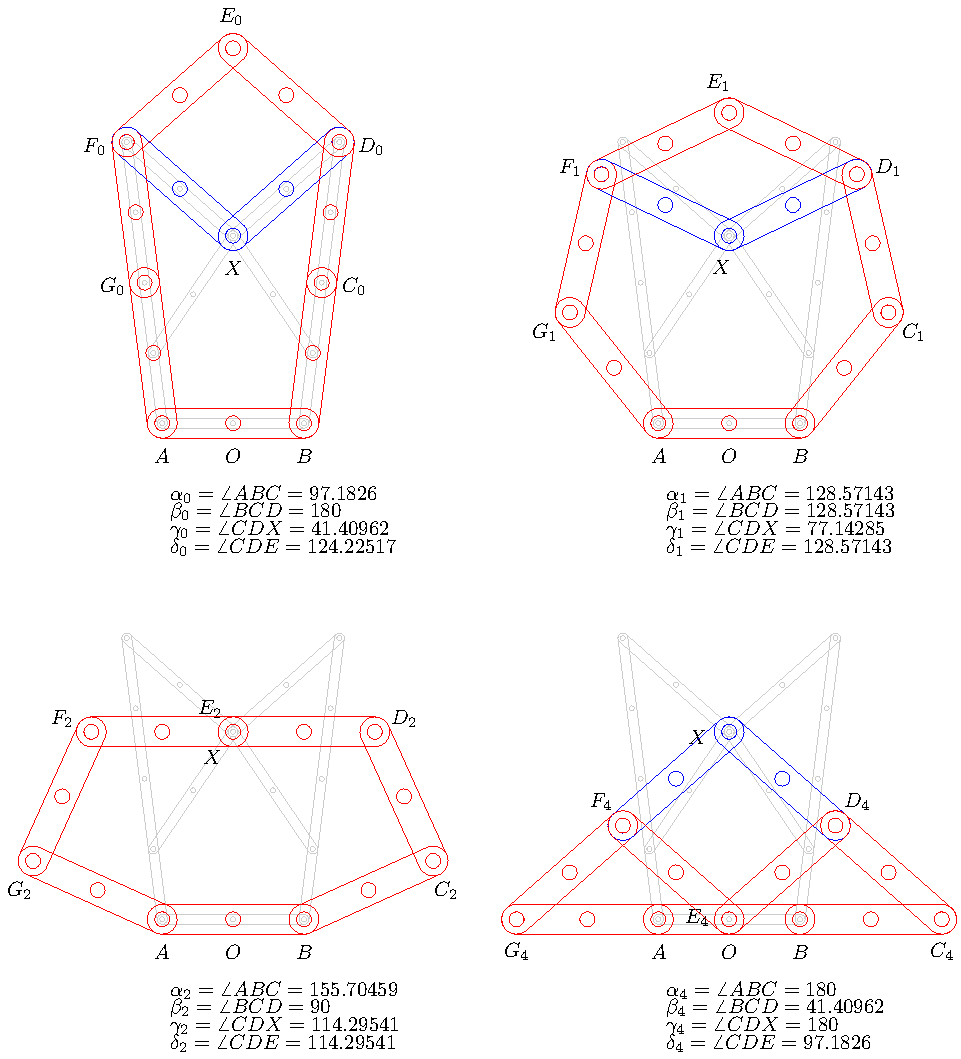
\includegraphics[scale=0.9]{builder/hepta-0}
\caption{Equilateral heptagons connected to rigid triangle $\triangle{ABX}$ in four positions. In red we have the perimeter $\overline{ABCDEF}$ in green two strips $\overline{DXF}$. In $(a)$ we have the heptagon as the tallest degenerated pentagon, in $(b)$ we have the regular heptagon, in $c$ we have a degenerated hexagon and in $(d)$ the shortest degenerated pentagon.}
\label{fig:build}
\end{figure}

Figure \ref{fig:build} show equilateral heptagons $ABCDEFG$ connected to the cluster of figure \ref{fig:build-base}. Vertices $A$ and $B$ are fixed while vertices $C$,$D$,$E$ and $F$ move. Is important to note that vertice $C$ positions $C_0,C_1,C_2,C_3$ follow the circular curve $C$ and vertice $D$ positions $D_0,D_1,D_2,D3$ follow the circular curve $D$.

The heptagon has two internal strips $\overline{DX}$ and $\overline{FX}$ connected to vertices $D$ and $F$ and to fixed vertex $X$.

We move the strips symmetrically. In figure $(a)$ we have the maximum extension to the top limited by fact that vertices $B$ and $D_0$ cannot be separated more since both are collinear with vertice $C_0$, being the angle $\beta_0 = \pi/2$.

From $(a)$ we reach state $(b)$ reducing $\beta$ until $\alpha_1 = \beta_1 = \delta_1 = 5\pi/7$ forming the regular heptagon.

From $(b)$ we reach state $(c)$ reducing $\beta$ until $\beta= \pi/2$.

In figure $(d)$ we reach the maximum extension to the bottom limited by the fact that vertices $X$ and $C_3$ cannot be separated more since both are collinear with vertice $D_3$, being the angle $\beta_3 = \arccos(3/4)$.

Table \ref{tbl:angles} show the values of angles $\alpha,\beta,\gamma,\delta$ for the positions $0,1,2,3$ corresponding to figures $(a),(b),(c),(d)$.

\begin{table}[H]
\begin{center}
\begin{tabular}{|c|c c c c|}
\hline
$Position$ & $\alpha$ & $\beta$ & $\gamma$ & $\delta$ \\ %[1ex]
\hline\
& \\[-1ex]
0 & $\phi+\psi$ & $\pi$ & $\theta$ & $2(\pi-\phi-\psi)-\theta$ \\[2ex] 
\hline
& \\[-1ex]
1 & $\dfrac{5\pi}7$ & $\dfrac{5\pi}7$ & $\dfrac{3\pi}7$ & $\dfrac{5\pi}7$ \\[2ex] 
\hline
& \\[-1ex]
2 & $\pi - \psi - \dfrac{\pi}4$ & $\pi/2$ & $\dfrac{\pi}4 - \psi$ & $\dfrac{\pi}4 - \psi$ \\[2ex] 
\hline
& \\[-1ex]
3 & $\pi$ & $\theta$ & $\pi$ & $\phi + \psi$ \\[2ex] 
\hline
\end{tabular}
\caption{Heptagon internal angles of positions $0-4$ shown in figure \ref{fig:build}.
Where $\theta$, $\phi$ and $\psi$ were defined in equations \ref{eq:theta}, \ref{eq:phi} and \ref{eq:psi} and shown in figure \ref{fig:build-base}. 
}
\label{tbl:angles}
\end{center}
\end{table}



\end{document}
